% \documentclass[preprint,12pt]{elsarticle}
% \usepackage{amssymb}
% \usepackage{amsfonts}
% \usepackage[utf8]{inputenc}
% \usepackage{graphicx}
% \usepackage{subcaption}
% \usepackage{xcolor}
% \usepackage{color}
% \usepackage{url}
% \usepackage{booktabs}

\definecolor{bluekeywords}{rgb}{0,0,1}
\definecolor{classgreen}{rgb}{0.17,0.57,0.68}
\definecolor{greencomments}{rgb}{0,0.5,0}
\definecolor{redstrings}{rgb}{0.64,0.08,0.08}
\definecolor{black}{rgb}{0,0,0}
\definecolor{blueattributes}{rgb}{0.37,0.52,0.62}
\definecolor{interfaceyellow}{rgb}{0.60,0.66,0.11}
\definecolor{directivepink}{rgb}{0.9,0.6,0.95}

\graphicspath{ {./crosscorr/src/img/} }


\chapter{Efficient GPU-accelerated Parallel Cross-correlation}

% \author{Karel Maděra}
% \ead{karelmad@email.cz}

% \author{Adam Šmelko}
% \ead{smelko@d3s.mff.cuni.cz}

% \author{Martin Kruliš}
% \ead{krulis@d3s.mff.cuni.cz}

% \affiliation{organization={Department of Distributed and Dependable Systems, Charles University},
%             city={Prague},
%             country={Czech Republic}}

% \begin{abstract}
% Cross-correlation is a data analysis method widely employed in various signal processing and similarity-search applications. Our objective is to design a~highly optimized GPU-accelerated implementation that would speed up the applications and also improve energy efficiency since GPUs could be more efficient than regular CPUs. There are two rudimentary ways to compute cross-correlation --- a definition-based algorithm that tries all possible overlaps and an algorithm based on the Fourier transform, which is much more complex but has better asymptotical time complexity. We have focused mainly on the definition-based approach which is better suited for smaller input data and we have implemented multiple CUDA-enabled algorithms with multiple optimization options. The algorithms were evaluated on various scenarios, including the most typical types of multi-signal correlations, and we provide empirically verified optimal solutions for each of the studied scenarios.
% \end{abstract}


% \begin{keyword}
%     cross-correlation \sep GPU \sep CUDA \sep parallel \sep algorithm \sep caching \sep optimizations
% \end{keyword}

% \end{frontmatter}

%% \linenumbers

%% main text

\section{Introduction}

Signal processing and analysis are essential in a plethora of applications ranging from video analysis, image matching, audio pattern recognition, or processing sensory inputs in various domains in physics, biology, pharmacy, or medicine~\cite{Kapinchev2015}. Cross-correlation is one of the basic methods employed in signal processing since it provides a metric that compares two signals and allows us to detect the best overlap including the relative shift between two signals.

In this work, we focus solely on the efficiency of the cross-correlation algorithm implementation and we aim to design optimizations that should speed up the computation. We tackle the problem with parallel computing, namely employing contemporary GPU accelerators which are particularly suited for data-parallel tasks. Although the task seems simple at first glance, achieving optimal efficiency is quite challenging due to the unique lock-step execution model of the GPUs which is placed in contrast with the workload imbalance that arises from a straightforward parallel implementation of cross-correlation. Furthermore, the GPUs often suffer from data-throughput issues which are raised by the fact the GPU memory needs to feed tens of thousands of computing cores; hence, we need to design an algorithm that promotes sharing loaded inputs among the cores by cleverly caching data in shared memory or registers. Having a highly optimized, GPU-accelerated implementation of cross-correlation can be beneficial for many applications, especially when the inputs are large or when they need to be processed in real-time. Furthermore, the GPU can achieve a better watt-to-performance ratio than the CPU when used efficiently, so our effort can contribute to power consumption savings in the long run.

Each application of cross-correlation has slightly different parameters, depending on the size of the correlated signals or the number of instances being computed simultaneously. For instance, computing one instance of cross-correlation of two large signals would use a different optimization algorithm than computing a correlation between one small signal and a long sequence of medium-sized signals (i.e., searching for a pattern in a video sequence). Thus, our second aim is to compare and analyze the most typical applications of cross-correlation and find the best algorithm for each type.

There are basically two approaches to computing a cross-correlation. A~na\"{i}ve (or definition-based) implementation that directly follows the mathematical definition (with time complexity of ${\cal O}(N^2)$, where $N$ is the size of both input signals) and an implementation that uses a Fourier Transform (FT) which has better asymptotical complexity (${\cal O}(N \log N)$), but also higher computational overhead. We are focusing solely on the definition-based implementations where the actual code optimizations can be explored and which is more suitable for computing multiple instances of smaller signals. The FT-based algorithm can be implemented using highly optimized libraries like cuFFT, which is currently not interesting from the perspective of basic research in parallel computing and optimizations. However, we have implemented a cuFFT version of cross-correlation as well so we can compare and evaluate both approaches empirically.


\subsection{Motivational application}\label{sec:intro-motivation}

Our research was motivated by material analysis --- detecting material defects by electron microscope. The method uses the microscope to scan the surface of a material in a raster pattern. It projects an electron beam towards individual points in the raster and collects a \emph{backscatter diffraction pattern} for each point. In computer science terms, the method collects a grey-scale image for each point in an input grid. For the selected material, there is a reference diffraction pattern that would be expected for a material without any defects. The collected images are compared with the reference image to detect possible distortions (e.g., translations, rotations, or warps) and these distortions can be interpreted as defects.

The comparison of measured and expected diffraction patterns is performed by dividing the images into multiple corresponding areas (i.e., areas with the same sizes and coordinates in both images) and cross-correlation is used to determine a relative shift of these two areas in the images. Thus we need to compute a cross-correlation of $N$ samples from one signal with $N$ samples from $M$ signals. The $N\cdot M$ easily reaches an order of millions, but the size of the areas is relatively small. Therefore, there is a lot of potential for parallelization, but it also means that the FT-based approach is likely to be slower than the definition-based approach.

Although the collection of the inputs from the microscope takes some time, the subsequent data processing can take even longer time when sequential implementation is used. Furthermore, in many cases, the results need to be re-computed multiple times with different input areas or different image-normalization preprocessing. Therefore, a GPU-accelerated implementation would significantly improve the user experience when interpreting the data.


\subsection{Contributions and outline}

We have implemented, measured, and analyzed a wide range of optimizations of four of the most typical cross-correlation applications. The main contributions can be summarized into three points:

\begin{itemize}
	\item We provide a CUDA-based algorithm (including an implementation) that is empirically evaluated as the best for each of the studied applications.
	\item Extensive evaluation and performance analysis of the individual optimization steps provide additional insight into GPU programming and code optimizations.
	\item We have determined the size thresholds of the input signals when the FT-based implementation (with better asymptotical complexity) takes over the definition-based implementation (which has lower overhead).
\end{itemize}

The source codes of the proposed algorithms, related scripts, and all the measured data as well as plotted graphs are available in a replication package in a GitHub repository\footnote{\url{https://github.com/asmelko/jpdc23-artifact}}.

The paper is organized as follows.
The definition of cross-correlation including the formalization of the studied instances is presented in Section~\ref{sec:cross}.
Section~\ref{sec:analysis} presents our analysis of parallelization possibilities and data re-use (inputs caching).
The proposed algorithms and their implementation details are described in Section~\ref{sec:algorithms} and empirically evaluated in Section~\ref{sec:crosscorr_experiments}.
Related work is overviewed in Section~\ref{sec:crosscorr_relwork} and Section~\ref{sec:crosscorr_conclusions} concludes the paper.

\section{Cross-correlation}\label{sec:cross}

First, we would like to review the mathematical definition of the cross-correlation (which is the basis for the definition-based implementation). Subsequently, we have selected and presented four of the most typical cross-correlation application types. Finally, we describe how the cross-correlation can be computed using Fourier transform.

% -----------------------------------------------------------------------------
\subsection{Definition}\label{sec:cross_corr_def}
% -----------------------------------------------------------------------------

Cross-correlation, also known as sliding dot product or sliding inner product, is a function describing the similarity of two series or two functions based on their relative displacement
% \citep{site:wiki_cross_corr}.
Cross-correlation of functions $f,g: \mathbb{C} \rightarrow \mathbb{R}$, denoted as \(f \star g\), is defined by the following formula:
\[
	(f \star g)(\tau) = \int_{-\infty}^{\infty} \overline{f(t)}g(t + \tau) \,dt,
\] 

where \(\overline{f(t)}\) denotes the complex conjugate of \(f(t)\) and \(\tau\) is the displacement of the two functions \(f\) and \(g\). In simpler words, the value \((f \star g)(\tau)\) tells us how similar the function \(f\) is to \(g\) when \(g\) is shifted by \(\tau\), with a higher value representing higher similarity.

For two discrete functions, as will be used in our case, cross-correlation of functions \( f, g: \mathbb{Z} \rightarrow \mathbb{R} \) is defined by the following formula:

\[
(f \star g)[m] = \sum_{i=-\infty}^{\infty} \overline{f[i]}g[i + m],
\] 


This definition of cross-correlation can be extended for use in two dimensions, as is required, for example, in image processing.
For two discrete functions \( f, g : \mathbb{Z}^2 \rightarrow \mathbb{R} \), cross-correlation is defined as:

\[
(f \star g)[m,n] = \sum_{i=-\infty}^{\infty} \sum_{j=-\infty}^{\infty} \overline{f[i,j]}g[i + m,j + n],
\]

Even though cross-correlation is defined on the whole $\mathbb{Z}$ for one dimension and $\mathbb{Z}^2$ for two dimensions, most use cases of cross-correlation work only on finite inputs, such as image processing working on finite images. The only values we are interested in are those where the two images overlap, which restricts the computation to $(w_1 + w_2 - 1) \cdot (h_1 + h_2 - 1)$ resulting values, where $w_i$ denotes the width and $h_i$ denotes the height of the image $i$.

This limits the part of the output we are interested in and leads us to the time complexity of the \textit{na\"{i}ve} definition-based algorithm. For each of the $(w_1 + w_2 - 1) \cdot (h_1 + h_2 - 1)$ output values, we need to multiply the overlapping pixel values and sum up all the multiplication results. There will be at most $min(w_1, w_2) \cdot min(h_1, h_2)$ overlapping pixels. For simplicity, let us work with two images of the same size $w \cdot h$. Then the time complexity of the definition-based algorithm is $(2w-1) \cdot (2h - 1) \cdot \mathcal{O}(w \cdot h)$, which gives us asymptotic complexity of $\mathcal{O}(w^2 \cdot h^2)$.


% -----------------------------------------------------------------------------
\subsection{Forms of cross-correlation}\label{sec:cross_corr_forms}
% -----------------------------------------------------------------------------

In cross-correlation applications, several forms of computation can be found. Each enables different types of optimizations, such as data caching and data reuse, batching, or precomputing. These forms differ in the number of inputs and in the way cross-correlation is computed between the inputs. The four basic forms are depicted in Figure~\ref{fig:cross_corr_forms}:

\begin{enumerate}
	\item one left input with one right input, in the rest of the thesis referred to as \textit{one-to-one} and depicted in Figure \ref{fig:cross_corr_one_to_one};
	\item one left input with many right inputs, referred to as \textit{one-to-many} and depicted in Figure \ref{fig:cross_corr_one_to_many};
	\item $n$ left inputs, \textbf{each one} cross-correlated with $m$ \textbf{different} right inputs (multiple instances of \textit{one-to-many}), referred to as \textit{n-to-mn} and depicted in Figure \ref{fig:cross_corr_n_to_mn};
	\item $n$ left inputs, \textbf{all} cross-correlated with \textbf{all} $m$ right inputs (full bipartite graph), referred to as \textit{n-to-m} and depicted in Figure \ref{fig:cross_corr_n_to_m}.
\end{enumerate} 

\begin{figure}[h]
	\centering
	\begin{subfigure}{0.4\textwidth}
		\centering
		\def\svgwidth{0.5\textwidth}
		\input{crosscorr/src/img/overlap-OneToOne.pdf_tex}
		\caption{one-to-one}
		\label{fig:cross_corr_one_to_one}
	\end{subfigure}
	\hfill
	\begin{subfigure}{0.4\textwidth}
		\centering
		\def\svgwidth{0.5\textwidth}
		\input{crosscorr/src/img/overlap-OneToMany.pdf_tex}
		\caption{one-to-many}
		\label{fig:cross_corr_one_to_many}
	\end{subfigure}
	\hfill
	\begin{subfigure}{0.4\textwidth}
		\centering
		\def\svgwidth{0.7\textwidth}
		\input{crosscorr/src/img/overlap-NtoMN.pdf_tex}
		\caption{n-to-mn}
		\label{fig:cross_corr_n_to_mn}
	\end{subfigure}
	\hfill
	\begin{subfigure}{0.4\textwidth}
		\centering
		\def\svgwidth{0.7\textwidth}
		\input{crosscorr/src/img/overlap-NToM.pdf_tex}
		\caption{n-to-m}
		\label{fig:cross_corr_n_to_m}
	\end{subfigure}
	
	\caption{Basic forms of cross-correlation}
	\label{fig:cross_corr_forms}
\end{figure}

The \textit{one-to-many} form is typical for applications where one sample (a~query) is located in a database or a time series of signal samples (e.g., in a~video sequence). Similarly, \textit{n-to-m} is merely an extension of this scenario where multiple queries are located in a database simultaneously \cite{Clark2011}. Perhaps the most unusual pattern is \textit{n-to-mn}. It has been inspired by the motivational application described in Section~\ref{sec:intro-motivation}. It is also an extension of \textit{one-to-many}, where both the query and the database samples are divided into corresponding sub-samples (e.g., areas with corresponding coordinates both in the query and database signals \cite{Kapinchev2015,zhang2015}). We have observed even more complex forms in the applications; however, they did not present any more opportunities for parallel processing or caching optimizations.

While each pair of input matrices can always be computed independently, the \textit{one-to-many}, \textit{n-to-mn} and \textit{n-to-m} types allow for the reuse of the left input matrix data for computation with multiple right input matrices. Additionally, the \textit{n-to-m} makes it possible to reuse data from the right matrix for computation with multiple left input matrices. 

For the same size of input data (i.e., $x$ left input matrices and $y$ right input matrices) the \textit{n-to-m} requires the computation of $x \cdot y$ pairs of matrices, compared to the \textit{n-to-mn} type which results in only $y$ pairs. The increased level of parallelism and increased arithmetic intensity allow for additional optimizations of the \textit{n-to-m} computation type compared to the \textit{n-to-mn} type. The \textit{one-to-one} and \textit{one-to-many} types are described separately, as compared to the general \textit{n-to-mn} or \textit{n-to-m} implementation, their implementations can more aggressively cache and reuse the left input matrix. 

Implementations of the two simpler types \textit{one-to-one} and \textit{one-to-many} can be extended to \textit{n-to-m} or \textit{n-to-mn} by running the simpler type of cross-correlation multiple times, possibly in parallel. Inversely, any implementation of either \textit{n-to-m} or \textit{n-to-mn} can be used to implement the two simpler types (with $n=1$). Another type that we could consider is the computation of a large number of independent pairs, which can be implemented by \textit{n-to-mn} (with $m=1$). A~large number of correlated pairs is a type not discussed further as it does not provide any additional opportunity for optimization compared to running the \textit{one-to-one} several times in parallel.



% -----------------------------------------------------------------------------
\subsection{Computation using Fourier transform}\label{sec:cross_corr_fft}
% -----------------------------------------------------------------------------

There is an alternate algorithm for computing cross-correlation based on the discrete Fourier transform (DFT). The asymptotic complexity of this algorithm (in two dimensions) is $\mathcal{O}(w \cdot h \cdot \log_2(w \cdot h))$, where $w$ is the width of each series and $h$ the height of each series. This improves on the asymptotic complexity $\mathcal{O}(w^2 \cdot h^2)$ of the definition-based algorithm described in the previous section, but the actual complexity constants are higher (thus, the FT-based implementation is better only for inputs larger than a certain threshold).

The Discrete Fourier transform can only be used to compute a special type of cross-correlation, the so-called \textit{circular} cross-correlation.
For a finite series $N \in \mathbb{N} \{x\}_n = x_0, x_1, ..., x_{N-1}, \{y_n\} = y_0, y_1, ..., y_{N-1}$, circular cross-correlation is defined as:

\[
(x \star_N y)_m = \sum_{i=0}^{N-1} \overline{x_m} y_{(m + i) \bmod N},
\]

where $\overline{x_m}$ denotes the complex conjugate of $x_m$.


Based on the Cross-Correlation Theorem~\cite{bracewell1966fourier}, the circular cross-correlation $(x \star_N y)_m$ can be computed using discrete Fourier transform (DFT) according to the following formula:

\[
(x \star_N y)_m = \mathbb{F}^{-1}(\overline{\mathbb{F}(x)}*\mathbb{F}(y))
\]

where $\mathbb{F}(x)$ and $\mathbb{F}(y)$ denote DFT of series $x$ and $y$ respectively, $\overline{\mathbb{F}(x)}$ denotes the complex conjugate of the DFT, $*$ denotes element-wise multiplication of two series and $\mathbb{F}^{-1}$ denotes inverse DFT.

To compute the non-circular (linear) cross-correlation of non-periodic series of size \textit{N}, we pad both series with \textit{N} zeros to the size \textit{2N}, as indicated in Figure \ref{fig:circular_cross_corr}. The results of circular cross-correlation are then the results of linear cross-correlation, only circularly shifted by $N-1$ places to the left with one additional 0 value at index $N$.

\begin{figure}[h]
	\centering
	\def\svgwidth{0.8\textwidth}
	\fontsize{9}{12}\selectfont
	\input{crosscorr/src/img/circular_cross_corr.drawio.pdf_tex}
	\caption{Comparison of linear and circular cross-correlation}
	\label{fig:circular_cross_corr}
\end{figure}


This process can be expanded into two dimensions, where the matrices are padded with \textit{N} rows and \textit{N} columns of zeros before being passed through 2D discrete Fourier transform. Here the circular shift of the results can be inverted by swapping the quadrants of the results while discarding row \textit{N} and column \textit{N}, which will be filled with zeros, as illustrated by Figure \ref{fig:quadrant_swap}. 

\begin{figure}[h]
	\centering
	\def\svgwidth{0.8\textwidth}
	\fontsize{9}{12}\selectfont
	\input{crosscorr/src/img/quadrant_swap.drawio.pdf_tex}
	\caption{The result quadrant swap}
	\label{fig:quadrant_swap}
\end{figure}


Based on this description, we can deduce the time complexity of the algorithm. For two matrices $a,b \in \mathbb{R}^{h \times w}$, the steps of the algorithm are:
\begin{enumerate}
	\item Padding $a_p, b_p \in \mathbb{R}^{2w \times 2h}$ of $a$ and $b$ with $w$ columns and $h$ rows of zeros in $\mathcal{O}(w \cdot h)$;
	\item The Discrete Fourier Transform (DFT) $A,B \in \mathbb{C}^{2w \times 2h}$ of $a_p$ and $b_p$ in $\mathcal{O}(w \cdot h \cdot \log_2(w \cdot h))$;
	\item Element-wise multiplication, also known as the Hadamard product, $C \in \mathbb{C}^{2w \times 2h}: C = \overline{A} \circ B$, where $\overline{A}$ the denotes complex conjugate of $A$, in $\mathcal{O}(w \cdot h)$;
	\item Inverse DFT $c \in \mathbb{R}^{2w \times 2h}$ of $C$ in $\mathcal{O}(w \cdot h \cdot \log_2(w \cdot h))$;
	\item Quadrant swap in $\mathcal{O}(w \cdot h)$
\end{enumerate}

In total, the steps described above give us an algorithm with asymptotic time complexity of $\mathcal{O}(w \cdot h \cdot \log_2(w \cdot h))$.

The FT-based algorithm will be used for comparison with the definition-based implementation. We have no ambition to optimize this algorithm further since the Fourier transform takes the most significant part and highly optimized libraries such as cuFFT\footnote{\url{https://docs.nvidia.com/cuda/cufft/}} already exist.

\section{Problem Analysis}\label{sec:analysis}

The design and implementation of an optimal solution are affected by several aspects of the problem. Furthermore, different scenarios of computing multiple signals being cross-correlated simultaneously benefit from different approaches. In this section, we provide an overview of the most important optimizations which are essential in our proposed algorithms.

For the sake of simplicity, we will focus solely on 2D cross-correlation since 1D correlation is significantly less interesting and all the proposed optimizations can be extended into higher dimensions easily. The input signals are discrete, so we will refer to the materialized inputs as \emph{matrices} to take advantage of the most familiar terminology available.


% -----------------------------------------------------------------------------
\subsection{Workload parallelization}\label{sec:analysis-workload}
% -----------------------------------------------------------------------------

A single cross-correlation (one-to-one) produces one output matrix, where each element corresponds to one possible relative shift between the input matrices. An example with two $4\times 4$ matrices is depicted in Figure~\ref{fig:cross_corr_shifts}. The value of the output element is computed as a sum of an element-wise multiplication performed on the overlapping area of the two input matrices.

\begin{figure}[ht]
	\fontsize{6}{8}\selectfont
	\centering
	\def\svgwidth{0.6\textwidth}
	\input{crosscorr/src/img/overlap-Shifts.pdf_tex}
	\caption{The output matrix with corresponding relative shifts of input matrices}
	\label{fig:cross_corr_shifts}
\end{figure}

The individual operations can be decomposed in a tree as indicated in Figure~\ref{fig:cross_corr_one_to_one_tasks}. The top-level node (green) represents the computation of a single output matrix. The second level (orange) represents computations of individual elements in the output matrix (different input overlaps). The third level (yellow) corresponds to the elementary multiplications performed on the overlapping area.

\begin{figure}[ht]
	\fontsize{5}{6}\selectfont
	\centering
	\def\svgwidth{0.65\textwidth}
	\input{crosscorr/src/img/overlap-Tasks.pdf_tex}
	\caption{A work decomposition of one-to-one cross-correlation}
	\label{fig:cross_corr_one_to_one_tasks}
\end{figure}

Both the first and the second levels comprise independent operations --- i.e., operations that can be performed without explicit data synchronization. The operations on the third level (multiplications) need to be reduced into the result at the second level (using a sum as the reduction operation). In case of more elaborate scenarios (\textit{one-to-many}, \textit{n-to-m}, and \textit{n-to-mn}), the tree in Figure~\ref{fig:cross_corr_one_to_one_tasks} is merely extended into a forest of independent trees, thus enabling another level of parallelism. Although this decomposition may indicate the problem is embarrassingly parallelizable, there are two major concerns for any GPU-accelerated implementation:

\begin{itemize}
	\item The workload at the second level is highly irregular. Corner elements are computed by a single multiplication whilst the elements in the center of the output matrix require a full element-wise multiplication and sum-reduction of the input matrices. This imbalance may cause serious code divergence (i.e., suboptimal performance) in the warps and thread blocks.
	\item The problem is highly data-bound as each loaded element is used in a simple elementary operation (multiplication and addition). This might create a significant underutilization of the GPU cores if each core spends most of the time waiting for the data.
\end{itemize}

Therefore, our objective is to design algorithms that will heavily reuse loaded input data whilst attempting to provide a better workload balance, especially at the warp level.


\subsubsection{Workload distribution}

One of the key aspects that affect the efficiency of GPU-based parallel programs is workload decomposition and distribution among the allocated threads. It defines the level of parallelism (since the threads are executed concurrently), synchronization (when one thread needs to wait for the results of another thread), and native parallel cooperation (via shared memory or warp-level instructions). It also affects registry allocation and, transitively, data reuse (since the input data needs to be moved from global memory to registers).

To simplify the description of the subsequent optimizations and algorithms (especially their approach to data reuse), we adopt the \emph{task} abstraction for the workload division and the work assignment to computing elements, where \emph{task} is usually an element of work performed by one CUDA thread.

\emph{Task} comprises a~well-defined group of nodes from the work decomposition schema introduced in Figure~\ref{fig:cross_corr_one_to_one_tasks}. The most straightforward implementation would map one \emph{overlap} (orange element at the second level) to one task and we denote this the \textbf{overlap-wise} (or simply the \textbf{overlap}) strategy. More elaborate task definitions, that would allow better input data reuse, will be outlined later using the overlap-wise strategy as the reference point.

In special cases, it is possible to assign each task to a group of threads (a~warp or a~block). This may provide a simpler approach to algorithms where more fine-grained division of tasks is impractical, but when each task may be processed in a cooperative or even SIMD-like manner. In the follow-up descriptions, we always assume that a task is assigned to one thread; unless we explicitly state otherwise.


% -----------------------------------------------------------------------------
\subsection{One-to-one data reuse}\label{sec:analysis-reuse}
% -----------------------------------------------------------------------------

The problem of the data-bound nature of the cross-correlation definition-based algorithm can be mitigated by smart caching of the input values which we generally refer to as \emph{data reuse}. In other words, every input value loaded into the registers or shared memory should be reused in multiple computations (multiplications) to improve the ratio between load and arithmetic instructions. In the following, we will introduce several task-forming strategies (i.e., how the cross-correlation individual operations are assigned to CUDA threads) that are designed to enable data reuse.

The most straightforward strategy (\textbf{overlap-wise}) assigns one relative input overlap (one sum of overlapping products) to a CUDA thread. Analyzing the input data access patterns, we have made an observation, that adjacent overlaps share significant portions of input data (as illustrated in Figure~\ref{fig:overlap_grouped_shared_data}).

\begin{figure}[ht]
	\centering
	\def\svgwidth{0.7\textwidth}
	\fontsize{7}{9}\selectfont
	\input{crosscorr/src/img/overlap-DataSharedByOverlaps.pdf_tex}
	\caption{Input data shared between neighboring overlaps}
	\label{fig:overlap_grouped_shared_data}
\end{figure}

The overlap-wise strategy can be implemented with data-reuse optimizations if the threads processing adjacent overlaps can share or exchange the input data efficiently (using shared memory or warp-shuffles). Another possibility is to create larger tasks that would aggregate multiple adjacent overlaps in a task so that a thread does not have to share the inputs with neighbors for data reuse as the reuse happens on loaded data internally. We have denoted this strategy \textbf{grouped-overlap}. For the sake of simplicity, we have selected only one dimension (which is depicted in Figure~\ref{fig:overlap_grouped_shared_data}) where the task aggregates the overlaps with the same relative column displacement and adjacent row displacements. We have considered more complex aggregations, but using a row-wise approach to grouping is much simpler to implement as we demonstrate later in Section~\ref{sec:grouped-overlap-alg}.
% TODO - warp shuffle v principu pouziva stejny princip ale col-wise. Nejak dopsat do textu.

% -----------------------------------------------------------------------------
\subsection{Fine grained parallelism}
% -----------------------------------------------------------------------------

In most cases (especially when multiple cross-correlations are computed simultaneously), the overlap-wise strategy gives us a sufficient amount of tasks to easily saturate the GPU. In fact, most of the data reuse strategies exploit some form of grouping --- i.e., one task groups computations of multiple overlaps together. In the case of smaller instances (especially in one-to-one cross-correlation), the total number of tasks may decrease so that the GPU is no longer entirely saturated. In such cases, we can choose a more fine-grained workload division. Each overlap computation is basically an element-wise sum of a Hadamard product of the overlapping part of the input matrices. The sum itself is associative, so we can compute the Hadamard product by multiple threads (concurrently) and then use a parallel sum reduction to get the result.

There are many ways to divide the Hadamard product, perhaps the most straightforward is to divide the matrix of products into stripes of adjacent rows (of a constant height, except for the last stripe). This strategy is denoted \textbf{split-row} and the height of the row stripes can be selected as a tuning parameter of the algorithm. Analogically, we define \textbf{split-col} strategy, which uses the same approach but creates stripes of columns instead of rows, and we refer to the principle of both strategies as \textbf{split-overlap}.

Technically, the split-overlap principle can be combined with the previously mentioned data reuse grouped-overlap; however, this often turns out to be counterproductive. The split-overlap is used in case the GPU is not saturated and in such cases, creating enough work for the threads is far more important than data reuse (i.e., the subsequent grouping of the overlap stripes does not improve the performance).

An alternative approach to split-overlap is to use basic overlap-wise task definition but assign a whole warp of threads per task. The warp divides the individual task elements (i.e., the products) among the threads evenly, while each thread accumulates its partial sum in its register. Finally, the threads employ warp instructions for the final reduction. This approach is used in a specialized \textbf{warp-per-overlap} algorithm (Section~\ref{sec:warp-per-overlap}).


% -----------------------------------------------------------------------------
\subsection{Processing multiple inputs simultaneously}\label{sec:analysis-multimat}
% -----------------------------------------------------------------------------

When multiple cross-correlations are being computed simultaneously (i.e., in \textit{one-to-many}, \textit{n-to-m}, and \textit{n-to-mn} scenarios), another level of data reuse becomes available. We can create tasks that aggregate computations using the same overlaps (relative dislocations) but on different input matrices. The main advantage is that the sizes of the overlapping inputs are exactly the same so this strategy does not negatively affect load balancing. Based on the application scenario, we have decided to explore two possible strategies:

\begin{figure}[ht]
	\centering	
	\begin{subfigure}{0.42\textwidth}
		\centering
		\def\svgwidth{\textwidth}
		\fontsize{7}{9}\selectfont
		\input{crosscorr/src/img/overlap-JobSizeOverlapSimple.pdf_tex}
		\caption{Grouping in \textit{one-to-many} configuration}
		\label{fig:job_size_modifiers_n_to_mn}
	\end{subfigure}
	\hfill
	\begin{subfigure}{0.42\textwidth}
		\centering
		\def\svgwidth{\textwidth}
		\fontsize{7}{9}\selectfont
		\input{crosscorr/src/img/overlap-JobSizeBoth.pdf_tex}
		\caption{Grouping in \textit{n-to-m} configuration}
		\label{fig:job_size_modifiers_n_to_m}
	\end{subfigure}
	
	\caption{Multi-matrix approach and its combination with overlap grouping}
	\label{fig:job_size_modifiers}
\end{figure}

\begin{itemize}
	\item \textbf{multi-matrix-right} uses multiple right matrices for each overlap (i.e., each value loaded from the left matrix is used in multiple correlations with right matrices). This approach will work in all three multi-matrix scenarios (\textit{one-to-many}, \textit{n-to-m}, and \textit{n-to-mn}).
	\item \textbf{multi-matrix-both} uses multiple left and right matrices so that each value from the left is used with all right matrices and vice versa. This approach is designed solely for the \textit{n-to-m} scenario.
\end{itemize}

Figure~\ref{fig:job_size_modifiers} shows the multi-matrix strategies and compares them with the grouped-overlap. Furthermore, the multi-matrix strategies can be combined with the grouped-overlap strategy as well as the split-overlap strategy.

\section{Proposed Solutions}\label{sec:algorithms}

We have experimented with various approaches to the problem and we present the best solution for each scenario. Most of the proposed solutions are based on a \emph{warp-shuffle algorithm} which was designed to embrace smart data caching in registers and their exchange among neighboring threads using warp-shuffle instructions. The algorithm can be improved by several data reuse and work distribution optimizations described in the previous section. The warp-shuffle algorithm is not very suitable for very small inputs, so we also present a \emph{warp-per-overlap} algorithm that prioritizes better workload distribution over data reuse which is critical when the GPU is not saturated by the warp-shuffle algorithm. The complete source codes are available in our replication package\footnote{\url{https://github.com/asmelko/jpdc23-artifact}}.

% -----------------------------------------------------------------------------
\subsection{Warp-shuffle algorithm}\label{sec:ws-algo}
% -----------------------------------------------------------------------------

The key principle of the warp-shuffle algorithm is that the threads within a warp\footnote{A group of $32$ consecutive threads executed in lock-step.} reuse data loaded from global memory into registers and employ warp-shuffle instructions to distribute the actual values. The same idea is behind the grouped-overlap reuse (depicted in Figure~\ref{fig:overlap_grouped_shared_data}), but in this case, the data reuse is col-wise rather than row-wise and it takes place in the registers of the entire warp (not the registers of a single thread) which need to be updated by warp-wise instructions (warp-shuffles).

First, we demonstrate the main principle using an overlap-wise strategy where the jobs are distributed among the treads so that each warp processes consecutive overlaps on the same row in the output matrix. In other words, the threads of a warp will process overlaps $[x,y], [x+1,y], \ldots, [x+31,y]$ (where $x$ is divisible by $32$). Figure~\ref{fig:warp-shuffle-principle} illustrates which data (from the left and the right matrix) are used by two adjacent threads from a warp if the overlapped area is traversed in row-major order.

\begin{figure}[ht]
	\centering
	\def\svgwidth{0.5\textwidth}
	\fontsize{8}{10}\selectfont
	\input{crosscorr/src/img/overlap-WarpShuffleShuffle.pdf_tex}
	\caption{Input data shared between neighboring overlaps}
	\label{fig:warp-shuffle-principle}
\end{figure}

A quick analysis reveals, that the data from both matrices can be shared among the threads. In the case of the left matrix, the value used by thread $1$ is required by thread $0$ in the subsequent iteration. In general, thread $i$ can load the value for the next iteration from thread $i+1$, so technically, the data are being shifted to the left among the threads. In the case of the right matrix, each thread requires the same value in the same iteration, except for the corner cases where a thread gets out of the bound of its overlapping area.


\subsubsection{Warp-wise buffers}

Data from both input matrices are cached in warp-wise buffers. A \emph{warp-wise buffer} is distributed among the registers of the individual threads in a round-robin manner and managed by warp-shuffle instructions. Each thread holds $N/32$ values, and value $i$ is kept in the $(i \bmod 32)$-th thread of the warp.

The left matrix is buffered in a $64$-item wide warp-wise buffer ($2$~registers per thread). Each thread $t$ finds its current value on the index $t$, which is coincidentally also stored in the register of thread $t$. After each step, the buffer is shifted to the left by one item using (two) warp-shuffle instructions. The reason for using the $64$-item wide buffer is to promote coalesced loading from the main memory (the data can be loaded in $32$-item wide transactions instead of one by one). With $64$ items, the buffer can be rotated $32\times$ without accessing main memory and after that, the second half of the buffer can be replenished with a single coalesced load.

The right matrix is buffered in a warp-wise buffer of $32$ items (one register per thread). This buffer does not require rotations, but the value required for each step needs to be loaded from the corresponding thread. This operation is also handled by a warp-shuffle instruction which can broadcast one value from the selected thread (i.e., its register) to all threads in a warp.

\begin{figure}[ht]
	\centering
	\def\svgwidth{0.9\textwidth}
	\fontsize{9}{12}\selectfont
	\input{crosscorr/src/img/warpshuffle-overview.pdf_tex}
	\caption{Buffering and data movements in warp-shuffle algorithm}
	\label{fig:warpshuffle-overview}
\end{figure}

Figure~\ref{fig:warpshuffle-overview} depicts data movements in $32$ consecutive steps. Note that each step comprises one arithmetic (FMA\footnote{Fused Multiply-Add --- i.e., an instruction computing $x*y+z$ expression.}) operation and three warp-shuffle instructions. At the end of the $32$-step block, both the gray part of the left buffer and the entire right buffer are filled with new data from the global memory in two coalesced transactions (when the entire warp loads a compact block of memory).


\subsubsection{Technical details}\label{sub:ws-technical-details}

There are several technical issues worth mentioning, albeit they are not essential for understanding the algorithm. The first one is how to handle corner cases, since the processed matrices are rarely aligned to the warp size and even if they are, the individual overlaps have different sizes. The loading of the inputs is handled in a way that values outside the input matrices are replaced with zeroes in the warp-wise buffers. Zeroes will not affect the cross-correlation results when used as inputs, so the only conditional code is in the loading step.

In the algorithm description, we have made a requirement, that consecutive items of the output matrix (on a row) are processed by a warp. In more detail, the thread block allocation is made so that the x-dimension has always size $32$ (represents threads within a warp), and the number of warps (the y-dimension) in a block is a tunable parameter of the algorithm (allowing us to find the best occupancy of the multiprocessors). Subsequent warps in a block operate on subsequent rows, which slightly improves the hit rate in hardware caches and also becomes beneficial in the follow-up optimizations. Furthermore, aligning the workload to the warp size also ensures that the edge case (when part of the warp is outside the output matrix) does not create any additional problems in the input buffering mechanism.

Finally, we made some special steps to ensure that the most internal loop of the algorithm (which performs exactly $32$ steps) is unrolled, so it can be highly optimized by the compiler (e.g., by resolving constant expressions in indices). The required hacks can be found in our source code.



% -----------------------------------------------------------------------------
\subsection{One-to-one optimizations}
% -----------------------------------------------------------------------------

The warp-shuffle algorithm can be improved by data reuse techniques described in Section~\ref{sec:analysis}. We shall start with optimizations that do not require multiple inputs (i.e., addressing \textit{one-to-one} configuration).

\subsubsection{Split-overlap}\label{sec:split-overlap-alg}

The split-overlap (specifically the split-row) optimization is designed for situations where the number of tasks is not sufficient to saturate the GPU and we need to decompose the workload further to enable another level of parallelism. The warp-shuffle algorithm is designed to be fully compatible with this optimization. The only difference is that multiple warps are allocated for tasks, that would be processed by a single warp in a regular overlap-wise strategy. The Hadamard product of each result is then computed by multiple threads, each of them being assigned the same amount of rows of the overlapping area (except for the last thread which may receive less). The product is both associative and commutative, so we can compute its part concurrently. Given the number of individual fragments is intended to be relatively low, aggregation by \texttt{atomicAdd} operation is quite adequate in this case.

We have experimented further with better and more complex work distribution patterns that could reduce the time when individual threads are idle due to code divergence caused by the irregularity of the workload. However, the overall improvement was barely measurable, possibly due to the fact the improvements were partially outweighed by increased overhead computations (calculating indices). Thus, we have concluded more elaborate solutions are not worth pursuing further, especially given the increase in their coding complexity.


\subsubsection{Grouped-overlap}\label{sec:grouped-overlap-alg}

If the inputs are sufficiently large, we can take an opposite path to optimizations that decrease the number of tasks due to grouping but promote data reusability further. The warp-shuffle approach already reduces global memory loads whilst making them more coalesced, but the data still needs to be shuffled among the threads. The profiling of basic overlap-wise implementation of the warp-shuffle algorithm confirms what is also apparent from Figure~\ref{fig:warpshuffle-overview} --- each FMA instruction (that performs the actual computation) requires $3$ warp-shuffle instructions (that just ensure the data are in the right registers). We can improve this ratio by grouping overlaps (each task comprises multiple overlaps) as suggested in Section~\ref{sec:analysis-reuse}. It enables caching multiple rows from both left and right matrices and subsequently using each value loaded in registers in multiple FMA operations.

\begin{figure}[ht]
	\centering
	\def\svgwidth{0.8\textwidth}
	\fontsize{9}{12}\selectfont
	\input{crosscorr/src/img/warpshuffle-grouped.pdf_tex}
	\caption{Data reuse in grouped-overlapped optimization (3 grouped overlaps)}
	\label{fig:warpshuffle-grouped}
\end{figure}

Figure~\ref{fig:warpshuffle-grouped} depicts a situation, where each task computes three overlaps displaced by one in the vertical direction ($[x,y]$, $[x,y+1]$, and $[x,y+2]$). The number of rows cached from the left matrix was also set to $3$ (although we may choose a different number of rows than the number of grouped overlaps, the best performance is usually achieved when they are the same). The number of the right rows needs to be set as the number of grouped overlaps and the number of left rows minus one ($3+3-1 = 5$). This setup was selected so all rows cached on the left are loaded exactly once (rows on the right are loaded multiple times).

In this particular case, a thread performs $9$ FMA instructions in each step while the registers are managed by $5$ broadcasts and $6$ shifts. In other words, the FMA to warp-shuffle instructions ratio was improved from $1:3$ to $9:11$. By increasing the grouping (and caching) factor, we can achieve better ratios of FMA to shuffle instructions. On the other hand, grouping reduces the number of tasks and increases the required amount of registers per thread, which may lead to low occupation of GPU cores. The best factor was determined empirically as $4$ overlaps per task.

Finally, there is one important implementation detail. Overlaps grouped together usually do not have the same size. As we iterate over the rows in the left matrix, the beginning or the end of the iteration needs to handle some corner cases. To reduce code divergence, we have divided the row-loop into three phases --- the \emph{init} phase, when the common overlapping part is growing, the \emph{main} phase, which was described above, and the \emph{final} phase, when the common overlapping part is diminishing. We have selected to implement the \emph{init} and the \emph{final} phases separately, to eliminate unnecessary conditions from the \emph{main} phase code (which is usually the dominant part of the calculation).


% -----------------------------------------------------------------------------
\subsection{Multiple cross-correlations}
% -----------------------------------------------------------------------------

Another level of parallelism and data reuse is opened when multiple cross-correlations are computed simultaneously. The warp-shuffle principle remains intact, but each task aggregates the same work from multiple cross-correlations (duplicating the necessary input buffers and the output values). The greatest advantage is that the computations are truly independent and they have identical shapes, so no additional corner cases have to be handled. The only requirement is that the matrices being correlated simultaneously have the same dimensions.

\subsubsection{Multi-matrix-right}

The first type assumes that one left matrix is correlated with multiple right matrices. This holds for \textit{one-to-many} and \textit{n-to-mn} scenarios. Technically, this assumption holds also for \textit{n-to-m} case, but we can do better optimizations with it as we demonstrate later.

\begin{figure}[ht]
	\centering
	\def\svgwidth{0.8\textwidth}
	\fontsize{9}{12}\selectfont
	\input{crosscorr/src/img/warpshuffle-multi-right.pdf_tex}
	\caption{Data reuse of multiple right matrices}
	\label{fig:warpshuffle-multi-right}
\end{figure}

Similarly to the grouped-overlap optimization, the objective is to improve the ratio between FMA instructions and warp-shuffle instructions. Increasing the number of right matrices by one adds one FMA instruction and one shuffle instruction as well, thus improving the ratio. In general, having $r$ right matrices cached simultaneously, the ratio of the instructions will be $r:r+2$ (i.e., approaching $1:1$ for large $r$ values).


\subsubsection{Multi-matrix-both}

In the case of \textit{n-to-m} scenario, we correlate multiple left matrices with multiple right matrices, so we can employ caching and data reuse on both sides. Unlike the case of the \emph{grouped-overlaps} optimization, all registers from the left buffer are multiplied with the broadcasted data from the right buffers which leads to $l\cdot r$ FMA operations per step (assuming $l$ and $r$ represents the amount of left and right cached matrices respectively). The details are depicted in Figure~\ref{fig:warpshuffle-multi-both}.

\begin{figure}[ht]
	\centering
	\def\svgwidth{0.8\textwidth}
	\fontsize{9}{12}\selectfont
	\input{crosscorr/src/img/warpshuffle-multi-both.pdf_tex}
	\caption{Data reuse when multiple matrices are used both on the left and the right}
	\label{fig:warpshuffle-multi-both}
\end{figure}

With this configuration, we can easily achieve a better ratio of FMA to shuffle instructions than $1:1$. For instance, in the case of $4$ left and $4$ right matrices being correlated in a joined effort, each thread will compute $4\times4=16$ FMA instructions for every $4\times 2 + 4 = 12$ shuffle instructions. On the other hand, each intermediate result requires a separate register where the products are accumulated, which can easily create register pressure if higher values of $l$ and $r$ are selected.


\subsubsection{Combining optimizations}

One of the greatest advantages of \emph{multi-matrix} extensions is that they are orthogonal to \emph{split-row} and \emph{grouped-overlap} optimizations --- in other words, we can combine these two techniques to improve performance further. The combination with the \emph{split-row} is completely straightforward and requires no special modifications. The combination with \emph{grouped-overlap} is slightly more difficult to imagine, so we include a visual aid.

\begin{figure}[ht]
	\centering
	\def\svgwidth{0.8\textwidth}
	\fontsize{9}{12}\selectfont
	\input{crosscorr/src/img/warpshuffle-combined.pdf_tex}
	\caption{Combining multi-matrix-both with grouped-overlap}
	\label{fig:warpshuffle-combined}
\end{figure}

Figure~\ref{fig:warpshuffle-combined} depicts the computation of a single thread when the two optimizations are combined. The input buffers are merely replicated in two dimensions --- i.e., multiple rows from multiple matrices are being cached. The most difficult part is to find the right balance of the parameters to achieve optimal performance.


% -----------------------------------------------------------------------------
\subsection{Warp-per-overlap algorithm}\label{sec:warp-per-overlap}
% -----------------------------------------------------------------------------

In the final part, we would like to revisit the problem of GPU underutilization when the matrices are very small. There is an alternate approach to the \emph{warp-shuffle} algorithm with \emph{split-row} optimization (described in Section~\ref{sec:split-overlap-alg}), which may provide even better performance since it aims specifically to better core occupation and minimization of code-divergence.

One of the greatest benefits and limitations of the warp-shuffle algorithm is the requirement that all threads in a warp must process adjacent overlaps within one row. Although it enables coalesced load and data shuffles, it also becomes a source of great thread divergence when the matrices are rather small, especially when the overlapping area width is comparable with the warp size, but not exactly matching. For instance, when correlating two $17\times 17$ matrices, the overlapping area is $33\times 33$, Hence, the second warp on each row will compute only one result value. This limitation is not mitigated by the split-row optimization.

An alternate approach is to allocate an entire warp to process each task --- a \emph{warp-per-overlap} algorithm. Using the basic overlap-wise task division, a task work is to iteratively process all compute elements of the Hadamard product of the overlapping area. The iteration can be divided in a vectorization manner and the threads will be assigned the FMA operations using the round-robin principle (Figure~\ref{fig:warp-per-overlap}).
 
\begin{figure}[ht]
	\centering
	\def\svgwidth{0.5\textwidth}
	\fontsize{7}{9}\selectfont
	\input{crosscorr/src/img/warp_per_shift-Basic.pdf_tex}
	\caption{The warp-per-overlap principle demonstrated on warps of size $4$}
	\label{fig:warp-per-overlap}
\end{figure}

This way, the workload is more evenly distributed among the threads of a warp which minimizes code divergence and maximizes the effective core occupancy. On the other hand, this task allocation does not provide any means for data reuse and the non-regular data access pattern will require much more global memory transactions.

We have experimented with several memory optimizations that will make the data loads more coalesced as well as manual caching of the input data in the shared memory. Although these improvements may be theoretically intriguing, they are not practical. The reason is that additional modifications of this algorithm increase the coding complexity quite a bit whilst improving the performance only when the input matrices are quite large. However, for larger input matrices the previously presented warp-shuffle algorithm exhibits better performance. Therefore, we propose the warp-per-overlap algorithm as an alternative to the split-row algorithm only for very small input matrices.

\section{Experimental Results}\label{sec:crosscorr_experiments}

To evaluate the performance of the proposed algorithms and optimizations, we performed extensive benchmarks covering the vast configuration space of optimization combinations, input sizes, and individual attuning parameters. In this section, we summarize the performance results of the described optimizations and compare them with each other to find the optimal one for each input size and problem configuration. In the end, we also compare our methods with the asymptotically better FFT-based algorithm to find the limits of definition-based algorithms.

% -----------------------------------------------------------------------------
\subsection{Experimental setup}
% -----------------------------------------------------------------------------

We carried out the experiments on three different NVIDIA GPUs representing three different architectures: Tesla V100 SXM2 32 GB (Volta arch.), Tesla A100 PCIe 80 GB (Ampere arch.), and Tesla L40 PCIe 48 GB (Ada Lovelace arch.). The systems were using CUDA 12.2 with driver version 535.104.05. Each single benchmark was repeated $10$ times, each time running for at least $0.1$ seconds. This setup was necessary to ensure proper measurement of short-running kernels. After removing the outliers, and checking that the remaining measurements have reasonable variance, the arithmetic mean of the remaining values was taken as the final result to be presented.

The results of all three GPUs do not differ significantly. The figures further presented in the paper cover only the results of the Tesla A100 GPU. The complete result set is available in our replication package\footnote{\url{https://github.com/asmelko/jpdc23-artifact}}.

\subsubsection{FFT-based algorithm}

In the following discussion, we also compare our proposed algorithms with the FFT-based approach. As described in Section~\ref{sec:cross_corr_fft}, the FFT-based algorithm runs in 5 steps: Input padding, Discrete Fourier Transform (DFT), Hadamard product, Inverse DFT and quadrant swap. We used highly optimized cuFFT routines for DFT and Inverse DFT. The Hadamard product was implemented in a custom kernel since it is an embarrassingly parallelizable algorithm. We chose to omit the quadrant swap from the measurements since this step is not generally required for all cross-correlation use cases (e.g. when the correlation result is processed further and the swap can be amortized in a subsequent step).

The DFT routines operate on a \emph{cuFFT plan} --- an opaque data structure, which needs to be initialized beforehand. Although we can only speculate what operations the plan initialization exactly performs, cuFFT documentation states that it also allocates GPU memory. The allocation is quite time-consuming in comparison to the kernel execution, so we decided to plot it separately to provide a more accurate picture of the relative performance. We plotted the FFT-based algorithm performance in two variants --- \emph{fft} aggregates the runtime of DFT, Hadamard product, and Inverse DFT; the \emph{fft+plan} also includes the time required for the plan creation. The \emph{fft+plan} presents a time that would be closer to a realistic application. The \emph{fft} shows the theoretical limits of the FFT-based approach that may be relevant if the initialization phase can be amortized or the cuFFT plan data structure can be re-used for many computations.
% Note, that comparing kernel runtimes to memory allocations is not generally fair, but in our case the allocation is an extra step in the FFT algorithm and therfore it is worthy the overall comparison.

% -----------------------------------------------------------------------------
\subsection{One-to-one benchmarks}
% -----------------------------------------------------------------------------

The one-to-one configuration can be solved using either the \emph{warp-shuffle} algorithm (possibly with the \emph{grouped-overlap} or \emph{split-row} optimization) or the \emph{warp-per-overlap} algorithm. First, we evaluate \emph{grouped-overlap} and \emph{split-row} optimizations separately to determine optimal tuning parameters. Afterward, we present the overall comparison of all methods including the na\"{i}ve \emph{overlap-wise} algorithm (baseline) and the FFT-based algorithm.

\subsubsection{Grouped-overlap}
%\paragraph{\textbf{\emph{grouped-overlap}}}

In this micro-benchmark, we present normalized times per single FMA operation (with amortized data transfers). To ensure reasonably interpretable values, we needed to saturate the GPU cores completely (i.e., generate enough workload even if the inputs are small). This prevents a misleading observation when an increase in the grouping factor (which improves efficiency) could be perceived as a decrease in the apparent FMA throughput just because the GPU gets undersaturated. We manually modified the kernel of the algorithm to run $4000$ copies of the input problem in a single grid. This allows us to correctly measure the actual FMA throughput, but the results are not directly comparable with other methods, especially in the case of very small inputs.

The results are shown in Figure~\ref{fig:grouped-overlap}. By increasing the number of grouped overlaps (and hence increasing the caching and data reuse factor), the optimization performs better for all matrix sizes. We can also observe that the algorithm performs significantly better for larger inputs, which is caused by the inherent limitation of the warp-shuffle principle. Very small matrices (like $16\times 16$) struggle with GPU underutilization and code divergence as the threads in a warp become idle for a considerable amount of time. With the larger inputs, the thread utilization becomes better and once exceeding $64\times 64$, the warp-shuffle algorithm can fully utilize the warp-wise buffer for the left matrix (as described in Section~\ref{sec:ws-algo}).

%We can also observe the diminishing effects of increasing the parameter values --- for $16\times 16$ matrix, a drastic data reuse of $8\times 8$ variant significantly reduces the number of jobs required to compute the output matrix. Since our implementation assigns output matrix computation to CUDA blocks, the number of participating threads in a block is bellow the optimal number of threads that are able to run in parallel on a single streaming multiprocessor.

% For bigger matrices, $8\times 8$ parameter variant starts to show the similar apparent speedup that the other variants. For matrices in the middle of the measured range, the speedup builds slower for $8\times 8$ than for the other variants because of the unfavorable initial+final phase to main phase ratio of \emph{grouped-overlap} algorithm.

% The figure also shows a rather big increase in FMA throughput for bigger matrices compared to the small ones. Very probably, this is caused by the warp-wise buffers. For small matrices, some registers in the $64$ registers-wide buffer will be unused while requiring the same number of costly global memory accesses. The buffer will reach the full utilization for $64\times 64$ matrices, which explains the steep slope ending at that data point. We still see the FMA throughtput increase and stabilize near $128\times 128$ sizes, caused by the stabilization of the internal ratio of global loads to buffer rotations mentioned in Section TODO.

For the sake of brevity, we do not show the plot measuring the influence of the block size on the performance of the algorithm (it is available in our replication package). The results conclusively show that as soon as the block size reaches a sufficient level to fully utilize a GPU streaming multiprocessor, the performance of the algorithm is not affected by increasing it further. Therefore, we used the block size of $4$ warps ($4\times 32$) for all the experiments.

\begin{figure}[ht]
	\begin{minipage}{.48\textwidth}
		\centering
		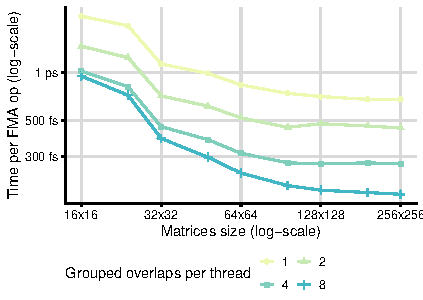
\includegraphics[width=\textwidth]{crosscorr/plots/one-to-one/grouped-overlap.pdf}
		\caption{The \emph{grouped-overlap} results, normalized times (per FMA) for completely saturated GPU}
		\label{fig:grouped-overlap}
	\end{minipage}%
	\begin{minipage}{.03\textwidth}~
	\end{minipage}
	\begin{minipage}{.48\textwidth}
		\centering
		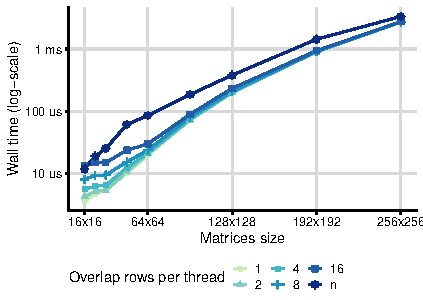
\includegraphics[width=\textwidth]{crosscorr/plots/one-to-one/split-row.pdf}
		\caption{The \emph{split-row} benchmark on various inputs, absolute (wall) times}
		\label{fig:split-row}
	\end{minipage}
\end{figure}

\subsubsection{Fine-grained parallelism}
% \paragraph{\textbf{\emph{split-row}}}

When problem size is not sufficient to saturate the GPU, a fine-grained parallelism is required. One possibility is to employ the \emph{split-row} optimization for the warp-shuffle algorithm, which splits each Hadamard product into multiple independently processed stripes. Figure \ref{fig:split-row} shows the performance for different job granularity levels ranging from the finest job of $1$ row per thread to $n$ (all) per thread (no splitting takes place --- i.e., referring to basic warp-shuffle implementation). As expected, the finest granularity helps the most for the smallest matrices and the speedup over $n$ (baseline) variant progressively diminishes as the input size increases (and thus saturates the GPU without splitting).

%\paragraph{\textbf{\emph{warp-per-overlap}}}
The alternate approach (\emph{warp-per-overlap} algorithm) has no tuning parameters, so we do not provide a separate micro-benchmark for it. The comparison of both algorithms is evaluated in the following.

\subsubsection{Comparison of all one-to-one solutions}
%\paragraph{\textbf{One-to-one optimizations comparison}}

Figure~\ref{fig:one-to-one} (left) summarizes the performance of the discussed one-to-one algorithms. The \emph{baseline} algorithm denotes the na\"{i}ve \emph{overlap-wise} implementation (one thread per one overlap with no data reuse) which we use as a baseline. Algorithms, which have tuning parameters, use their optimal values for given input sizes (as determined in the previous micro-benchmarks).

\begin{figure}[ht]
	\centering
	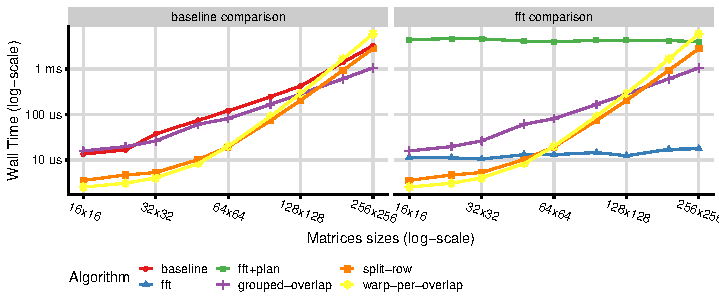
\includegraphics{crosscorr/plots/one-to-one/one-to-one.pdf}
	\caption{Comparison of one-to-one algorithms}
	\label{fig:one-to-one}
\end{figure}

The \emph{grouped-overlap} optimization is the most beneficial for larger matrices while for smaller matrices it suffers the low GPU occupancy due to the insufficient amount of tasks. The \emph{split-row} and \emph{warp-per-overlap} algorithms perform better on smaller matrices as they resolve the occupancy issue. The \emph{warp-per-overlap} performs better on very small inputs as it was designed specifically to prefer core occupancy over data caching. The \emph{split-row} optimization of the \emph{warp-shuffle} algorithm performs slightly worse for matrices smaller than $64\times64$; for larger matrices, the data reuse and coalesced loads become more important, so it outperforms \emph{warp-per-overlap}. Overall, the proposed optimizations perform better than baseline \emph{overlap-wise} algorithm, being $5.3\times$ faster for $16\times16$ input and $3.1\times$ faster for $256\times 256$ input.

% \paragraph{\textbf{Comparison with FFT}}

%Finally, we compare the proposed optimizations against the FFT-based algorithm, in our case the highly optimized CUDA library \emph{cuFFT}~\cite{site:cufft}. Recalling from Section~\ref{sec:cross_corr_fft}, FFT based algorithm must perform the input padding, Discrete Fourier Transform (DFT), Hadamard product, Inverse DFT and quadrant swap. We used cuFFT optimized routines for DFT and Inverse DFT. For Hadamard product, we implemented the custom kernel (Hadamard product is an embarrassingly parallelizable algorithm and its implementation details were omitted for brevity).

%In order to provide less convoluted and fairer results, we decided not to include padding and quadrant swap into the benchmark. We chose to omit the quadrant swap because this step is not generally required for every cross-correlation usecases; e.g., in digital image cross-correlation, only the maximum of the cross-correlation matrix is needed. Skipping quadrant swap therefore makes it more fair comparison with definition-based algorithms. Regarding the paddings, it is a simple operation that may influence the performance very little, so we omitted it for the simplicity of the benchmarking code.

%The DFT routines operate on a \emph{cuFFT plan} --- an opaque data structure, which needs to initialized beforehand. Although we can only speculate what operations does plan initialization exactly performs, cuFFT documentation states that it allocates GPU memory. The allocation takes multiple magnitudes longer than the kernel runtimes, so we decided to plot it separately to provide the better picture of the speedups. We plotted FFT-based algorithms in two variants --- \emph{fft}, which shows the aggregated runtime of DFT, Hadamard product and Inverse DFT, and \emph{fft+plan}, which also adds the plan creation to the sum. Note, that comparing kernel runtimes to memory allocations is not generally fair, but in our case the allocation is an extra step in the FFT algorithm and therfore it is worthy the overall comparison.

The right part of Figure~\ref{fig:one-to-one} reveals that the cuFFT plan creation is the most costly part of the algorithm, dominating the runtime in each measured data point. When the initialization is taken into account, the definition-based approach appears much better in the terms of performance. The turning point, where the \emph{fft+plan} surpasses our optimizations, seems to be around $384\times 384$ matrix. When considering \emph{fft} alone, only the \emph{warp-per-overlap} algorithm outperforms it (having $4.5\times$ speedup on $16\times 16$ inputs) and the turning point is around $48\times 48$.


% -----------------------------------------------------------------------------
\subsection{One-to-many benchmarks}
% -----------------------------------------------------------------------------

The \emph{one-to-many} and \emph{n-to-mn} scenarios enable utilization of the \emph{multi-matrix-right} optimization of the warp shuffle algorithm. This optimization can be combined with \emph{grouped-overlap} or \emph{split-row}, so we present their respective performance evaluation in detail.

We did not include the \emph{warp-per-overlap} evaluation in this section, because it does not provide any additional improvement in terms of performance. The additional workload of multiple cross-correlations mitigates the need for extremely fine-grained parallelism, so the \emph{split-row} optimization is more than sufficient even for the smallest matrices.

\subsubsection{Multi-matrix-right with grouped-overlap}
% \paragraph{\textbf{\emph{multi-matrix-right grouped-overlap}}}

In this configuration, we are benchmarking the one-to-many scenario with $4000$ right matrices, which completely saturates the GPU. The left subplot of Figure~\ref{fig:multimat-right-grouped-overlap} shows the \emph{grouped-overlap} results without the \emph{multi-matrix-right} optimization. In the middle and the right subplot, the number of right matrices per thread is $2$ and $4$ respectively (i.e., enabling the multi-matrix caching). The results indicate that increasing the number of right matrices per thread does not collide with the data reuse made by the \emph{grouped-overlap} optimization and both optimizations can work in synergy.

\begin{figure}[ht]
	\centering
	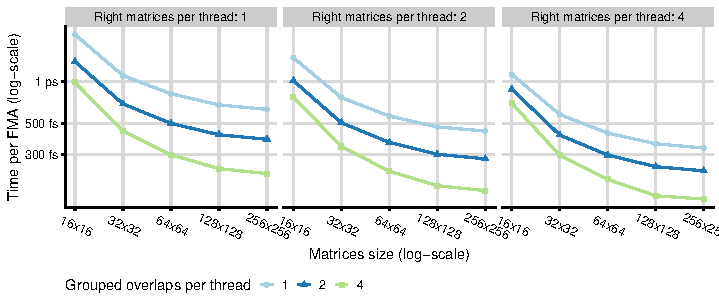
\includegraphics{crosscorr/plots/one-to-many/multimat-right-grouped-overlap.pdf}
	\caption{\emph{Multi-matrix-right}+\emph{grouped-overlap} results (one-to-many, $4000$ right matrices)}
	\label{fig:multimat-right-grouped-overlap}
\end{figure}

Considering a sufficient total number of the right matrices, we can increase the factor of right matrices per thread significantly more and still expect the performance to improve. The primary limitation is the maximum number of registers per thread a GPU allows to allocate. The required number of registers increases linearly with the product of right matrices per thread used by \emph{multi-matrix-right} and warp-wise buffers used by the \emph{grouped-overlap} (which is about $3 \cdot 4^2$ registers per thread for the variant that reuses the data the most intensively in Figure~\ref{fig:multimat-right-grouped-overlap}). When the maximum is exceeded, the GPU resorts to register spilling (offloading to local memory), which harms the performance significantly.

We have observed that the parameter values presented in Figure~\ref{fig:multimat-right-grouped-overlap} are in a reasonable range. Increasing the grouping factor or number of right matrices further does not help much with performance on current GPU architectures, but it creates additional issues with the compilation (especially bloating the size of our artifact). Hence, we have excluded higher values from the presented results for practical reasons.


\subsubsection{Multi-matrix-right with split-row}
% \paragraph{\textbf{\emph{multi-matrix-right split-row}}}

This micro-benchmark was designed to determine how the combination of multi-matrix data reuse and fine-grained parallelism can improve performance. In theory, applying \emph{multi-matrix-right} on small inputs may decrease the performance because it groups tasks, thus limiting the parallelism. Combining multi-matrix optimization with \emph{split-row} may provide enough parallel GPU work whilst improving the data reuse.

\begin{figure}[ht]
	\centering
	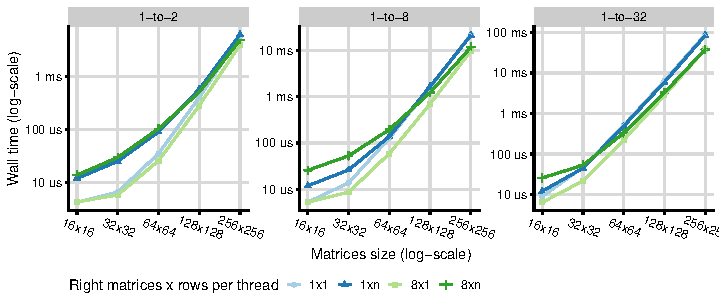
\includegraphics{crosscorr/plots/one-to-many/multimat-right-split-row.pdf}
	\caption{\emph{Multi-matrix-right}+\emph{split-row} benchmark results (please note that the $8\times1$ and $8\times n$ parametrizations are in fact $2\times1$ and $2\times n$ in the \emph{1-to-2} scenario since we can cache only up to the total number of right matrices)}
	\label{fig:multimat-right-split-row}
\end{figure}

%We ploted the optimization combination in Figure~\ref{fig:multimat-right-split-row}. If we compare only \emph{multi-matrix-right} optimization without \emph{split-row} (a triangle and a cross in each subplot), we can see that a big data reuse (cross) decreases the performance for small matrix sizes. But if we look at their \emph{split-row} alternatives (a circle and a square in each subplot), we can see that finer sized jobs counter the performance degradation caused by the data reuse. Ultimately, when the problem size is bigger and a GPU is saturated, these alternatives meet (circles meet with triangles and squares meet with crosses) and the performance is the same.
Figure~\ref{fig:multimat-right-split-row} demonstrates how the \emph{split-row} improves performance for small problem sizes. The $1\times n$ and $8\times n$ denote the versions that do not take advantage of \emph{split-row} (the size of row-stripes is $n$, which stands for the size of the overlapping area). The $1\times 1$ and $8\times 1$ stand for the most fine-grained versions of \emph{split-row} (one task takes only one row). The data indicate that in the extreme, the speedup caused by splitting the rows could reach an order of magnitude ($16\times16$ with a low number of right matrices). Furthermore, the $8\times 1$ parametrization (i.e., the most fine-grained division that caches $8$ right matrices) exhibits the best performance over the examined domain.

\subsubsection{Comparison of one-to-many optimizations}
%\paragraph{\textbf{One-to-many optimizations comparison}}

The overall comparison is presented in Figure~\ref{fig:one-to-many}. Similarly as for one-to-one optimizations, the \emph{split-row} dominates the small matrices and \emph{grouped-overlap} dominates the larger matrices. Employing \emph{multi-matrix-right} (especially when combined with \emph{split-row}) shifts the turning point where higher data reuse wins over more granular jobs. Using $32$ right matrices, we achieve $11.8\times$ speedup over na\"{i}ve \emph{overlap-wise} (baseline) algorithm for $16\times 16$ input and $6\times$ speedup for $256\times 256$ input.

When we compare the best definition-based algorithm with cuFFT, the \emph{split-row} still outperforms \emph{fft} for extra small matrices. The turning point for \emph{fft+plan} is slightly beyond the size of $256\times 256$ for $2$ input matrices, and $128\times 128$ for $32$ input matrices.

\begin{figure}[ht]
	\centering
	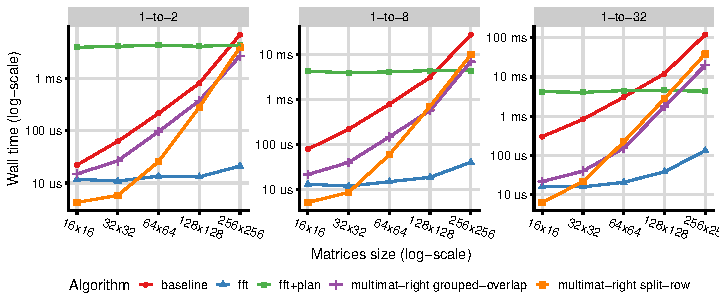
\includegraphics{crosscorr/plots/one-to-many/one-to-many.pdf}
	\caption{Comparison of one-to-many algorithms}
	\label{fig:one-to-many}
\end{figure}


\subsubsection{Extending one-to-many into n-to-mn}

The \emph{n-to-mn} problem is in fact $n$ instances of \emph{one-to-many} problem. There are two ways of extending the \emph{one-to-many} implementation --- we could either simply run the original kernel $n$ times simultaneously or create a new kernel that takes an additional index. After a careful analysis, we found no additional benefits of implementing a separate kernel. When running \emph{one-to-many} kernel $n$ times, the only issue worth mentioning is that the runtime must utilize a sufficient amount of CUDA streams, so the execution of the kernels may overlap in case the individual invocations cannot saturate the GPU.

The overhead of the simultaneous kernel execution is negligible, so we have omitted figures with the performance results from the paper for the sake of brevity. The data and the plots may be found in the attached replication package.


% -----------------------------------------------------------------------------
\subsection{n-to-m benchmarks}
% -----------------------------------------------------------------------------

This scenario allows the most elaborate data reuse pattern called the \emph{multi-matrix-both} optimization. Similarly to \emph{multi-matrix-right}, it can be combined with \emph{grouped-overlap} or \emph{split-row}.

\subsubsection{Multi-matrix-both with grouped-overlap}
%\paragraph{\textbf{\emph{multi-matrix-both grouped-overlap}}}

In Figure~\ref{fig:multimat-both-grouped-overlap}, we present the results of \emph{grouped-overlap} alone (left subfigure), combined with \emph{multi-matrix-right} (center subfigure), and with \emph{multi-matrix-both} (right subfigure). Regardless of the number of grouped overlaps, the \emph{multi-matrix} optimization alone improves the speedup, and the combination of both optimizations exhibits the best performance. In the case of the highest overlap grouping, the speedup of \emph{both} variant over \emph{right} variant is about $1.75\times$ on all input sizes.

\begin{figure}[ht]
	\centering
	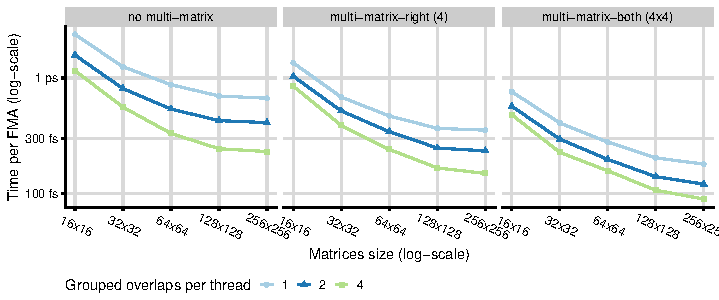
\includegraphics{crosscorr/plots/n-to-m/multimat-both-grouped-overlap.pdf}
	\caption{\emph{Multi-matrix-both}+\emph{grouped-overlap} benchmark results ($128$-to-$128$ matrices)}
	\label{fig:multimat-both-grouped-overlap}
\end{figure}


\subsubsection{Multi-matrix-both with split-row}
%\paragraph{\textbf{\emph{multi-matrix-both split-row}}}

Similarly to \emph{multi-matrix-right} combination, we aim at verifying that \emph{split-row} optimization enables the data reuse on smaller matrices without any performance downgrade. We tested this on two different matrix counts: $2$-to-$2$ and $8$-to-$8$ matrices (top and bottom pair of subfigures in Figure~\ref{fig:multimat-both-split-row} respectively). The results indeed show that for small matrices, the \emph{multi-matrix} alone (the left pair of subfigures) is slower than the \emph{multi-matrix} combined with \emph{split-row} (the right pair of subfigures). The speedup of finer parallelism for $16\times16$ matrix and the highest --- about $5\times$. As expected, the speedup gets negligible for larger matrices.

\begin{figure}[ht]
	\centering
	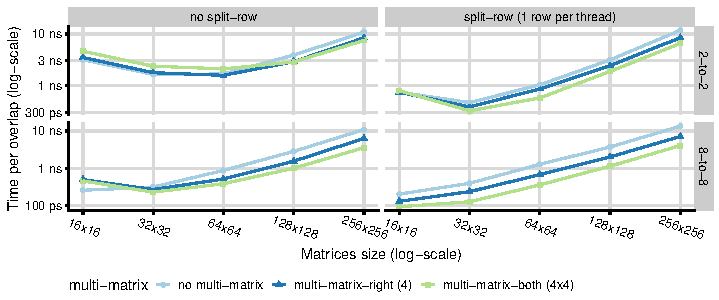
\includegraphics{crosscorr/plots/n-to-m/multimat-both-split-row.pdf}
	\caption{\emph{Multi-matrix-both}+\emph{split-row} benchmark results}
	\label{fig:multimat-both-split-row}
\end{figure}

\subsubsection{Comparison of n-to-m optimizations}
%\paragraph{\textbf{n-to-m optimizations comparison}}

The overall comparison is presented in Figure~\ref{fig:n-to-m}. Similarly to \emph{one-to-many} optimizations, the \emph{split-row} dominates smaller inputs while \emph{grouped-overlap} dominates larger inputs. However, when the multi-matrix factor gets higher ($32$-to-$32$ matrices), the \emph{grouped-overlap} gets more efficient than \emph{split-row} as the GPU is already saturated and data reuse becomes more important.

Another observation is that cuFFT gets better even for slightly smaller matrices when the number of cross-correlations is growing. That is a natural conclusion of the fact that the cuFFT plan initialization takes constant time, so it gets more amortized into the overall computation. For $32$-to-$32$ matrices, the turning point gets as low as $64\times 64$ matrices.

\begin{figure}[ht]
	\centering
	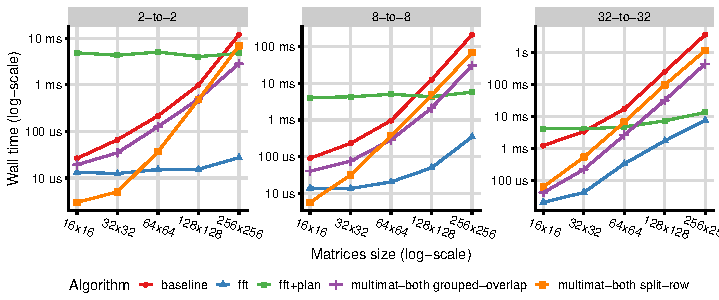
\includegraphics{crosscorr/plots/n-to-m/n-to-m.pdf}
	\caption{Comparison of n-to-m algorithms on various inputs.}
	\label{fig:n-to-m}
\end{figure}


% -----------------------------------------------------------------------------
\subsection{Summary and outcomes}
% -----------------------------------------------------------------------------

To summarize the empirical results, we provide basic guidelines for selecting the optimal algorithm and its optimization. Table~\ref{tab:overview-all} presents the algorithm of choice for given scenarios (rows) and matrix sizes (columns). The \emph{one-to-many} instances implicitly assume utilization of \emph{multi-matrix-right} optimization and the \emph{n-to-m} always employ \emph{multi-matrix-both} optimization.

As indicated in the previous benchmarks, the smallest configurations benefit from \emph{split-row} optimization (or the \emph{warp-per-overlap} algorithm, in case of \emph{one-to-one} scenario). The middle-sized problems can benefit from the \emph{grouped-overlap} optimization and the largest problems should switch to the FFT-based approach which is asymptotically better.

Please note that the turning points for each configuration are not exact and they may differ slightly across the GPU architectures.

\begin{table}
	\begin{tabular}{l|cccccccc}\toprule
		             & $16^2$                                     & $32^2$                                & $64^2$                                & $128^2$         & $192^2$                     & $256^2$ & $384^2$ & $\infty$ \\\midrule
		\emph{1-to-1}   & \multicolumn{3}{c|}{\texttt{warp-overlap}} & \multicolumn{1}{c|}{\texttt{split}}   & \multicolumn{3}{c|}{\texttt{grouped}} & \multicolumn{1}{r}{\texttt{fft+p}}                                \\\bottomrule
		\emph{1-to-2}   & \multicolumn{4}{c|}{\texttt{split}}        & \multicolumn{2}{c|}{\texttt{grouped}} & \multicolumn{2}{c}{\texttt{fft+p}}                                                                        \\
		\emph{1-to-8}   & \multicolumn{3}{c|}{\texttt{split}}        & \multicolumn{2}{c|}{\texttt{grouped}} & \multicolumn{3}{c}{\texttt{fft+p}}                                                                        \\
		\emph{1-to-32}  & \multicolumn{2}{c|}{\texttt{split}}        & \multicolumn{2}{c|}{\texttt{grouped}} & \multicolumn{4}{c}{\texttt{fft+p}}                                                                        \\\bottomrule
		\emph{2-to-2}   & \multicolumn{4}{c|}{\texttt{split}}        & \multicolumn{2}{c|}{\texttt{grouped}} & \multicolumn{2}{c}{\texttt{fft+p}}                                                                        \\
		\emph{8-to-8}   & \multicolumn{3}{c|}{\texttt{split}}        & \multicolumn{2}{c|}{\texttt{grouped}} & \multicolumn{3}{c}{\texttt{fft+p}}                                                                        \\
		\emph{32-to-32} & \multicolumn{4}{c|}{\texttt{grouped}}      & \multicolumn{4}{c}{\texttt{fft+p}}                                                                                                                \\\bottomrule
	\end{tabular}
	\centering
	\caption{Overview of the best algorithms (and optimizations) for individual scenarios and input sizes}
	\label{tab:overview-all}
\end{table}

\section{Related Work}\label{sec:crosscorr_relwork}

% Projit nize uvedene a dat je nejak do perspektivy pripadne chronologicke navaznosti
% Same as with the previously mentioned work, these approaches solve a slightly different problem with regards to data reuse since they share the intermediate results between workers, while we reuse only the global memory loads. But the idea of grouping multiple overlaps into a single job is the same.

% There are plenty of other scientific papers related to GPU cross-correlation~. However, they describe GPU optimizations for a specific scientific use-case and use almost exclusively some modifications of the asymptotically better FFT-based algorithms. Therefore, the optimizations mentioned in these works are not applicable to our problem.

% unsorted
% --------

% general template matching
% 2d cross correlation implemented using FFT
% \cite{liu2011gpu} - Gpu accelerated fourier cross correlation computation and its application in template matching

% Optical coherence tomography
% 2d
% used in ophtalmology, where detailed imagery of the retina, the optic nerve, and other parts of the eye is essential for accurate diagnosis 
% \cite{Kapinchev2015} - GPU implementation of cross-correlation for image generation in real time

% particle image velocimetry - CC is used to compute displacement vectors
% process has high complexity and is optimized using GPU cuFFT
% \cite{zeng2022gpu} - PU-accelerated MART and concurrent cross-correlation for tomographic PIV (2022, asi aplikacni)

% Digital image correlateion
% 2d
% \cite{zhang2015} - High accuracy digital image correlation powered by GPU-based parallel computing

% seismic:
% --------------

% ambient noise imaging uses noise CC functions to obtain earth underground structures
% due to increasing number of seismomenters and the data they produce, getting more accurate earth's seismic information is limited by the runtime of NCF
% authors optimize it on GPU 
% \cite{zhou2021high} - A High Performance Computing Method for Noise Cross-Correlation Functions of Seismic Data

% another seismic usecase for GPU cross correlation
% \cite{beauce2017fast} - Fast Matched Filter (FMF): An Efficient Seismic Matched‐Filter Search for Both CPU and GPU Architectures

% PCC is used for Interstation correlation, which is the basic operation in seismic noise and coda-wave interferometry
% PCC has high computational complexity, authors rewrite it in terms of complex FFT and provide GPU impl
% \cite{ventosa2019towards} - Towards the processing of large data volumes with phase cross-correlation (2019, aplikacni)

% stereo vision:
% ---------------

% authors introduce optimized algorithms and provide real-time GPU implementation of disparity map computation used in autonomous vehicle applications
% 2d
% \cite{fan2017real} - Real-time implementation of stereo vision based on optimised normalised cross-correlation and propagated search range on a gpu (2017, aplikacni)
% \cite{syed2021accelerated} - Accelerated Stereo Vision Using Nvidia Jetson and Intel AVX
% \cite{chang2022efficient} - Efficient stereo matching on embedded GPUs with zero-means cross correlation

% astronomy:
% ----------

% signal processing for radio astronomy
% % 1d
% \cite{Clark2011} - Accelerating Radio Astronomy Cross-Correlation with Graphics Processing Units
% \cite{ord2015murchison} - The Murchison widefield array correlator
% \cite{ragoomundun2020cublas} - A cuBLAS-based GPU correlation engine for a low-frequency radio telescope

% Many works leverage some form of partitioning cross-correlation problem into tasks to be executed in parallel. Khalil et al.~\cite{khalil2013accelerating} distributes the work of 1D cross-correlation between nodes in a local network. The sequence of all delays (overlaps in our terminology) is `sliced' and distributed according to the number of nodes and their computing power. In our work, we employ the same distribution technique but with a difference of much finer granularity, dividing work into single overlaps or even into parts of overlaps between workers.

Cross-correlation relates to the problem of signal processing in many different fields and we have collected several examples where the GPU processing creates an edge. In the domain of radio astronomy, all signals from radio antennas need to be usually correlated with each other, which puts this problem in the HPC domain. Various cross-correlation optimizations have been proposed: Clark et al.~\cite{Clark2011} developed a GPU kernel, which promotes tiling and optimized memory transfer. By utilizing both FPGAs and GPUs, Ord et al.~\cite{ord2015murchison} propose a hybrid approach to achieve sufficient performance. Ragoomundun et al.~\cite{ragoomundun2020cublas} utilize batched matrix multiply routines of the cuBLAS GPU library to implement their optimized correlator to enable real-time processing for telescopes.

Seismic interferometry is another use case, where cross-correlation plays a major role. An increasing amount of seismometers allows the production of more detailed seismic information of the Earth but it is typically limited by the processing runtime. Zhou et al.~\cite{zhou2021high} optimize noise cross-correlation functions used to obtain Earth's underground structures. Ventosa et al.~\cite{ventosa2019towards} implement a GPU version of phase cross-correlation, which is used in Interstation correlation. Beaucé et al.~\cite{beauce2017fast} discuss optimizations of Fast Matched Filter, which is an important tool in the detection of seismic events.

Applications of cross-correlation can be also found in computer vision. Fan et al. discuss autonomous vehicle applications in the context of disparity maps~\cite{fan2017real} (used for stereo vision) or lane detection~\cite{fan2018real}. Typically, mobile platforms such as autonomous cars and robots have strict limits to their power intake, so Syed et al.~\cite{syed2021accelerated} and Chang et al~\cite{chang2022efficient} described ways to further optimize stereo vision algorithms on embedded hardware, such as Nvidia Jetson GPU, to achieve the required speed of processing while maintaining low power consumption.

It has been established that fast cross-correlation is useful in various practical domains. However, most of the papers mentioned in the previous put little effort into the optimizations of the algorithm and provide only straightforward GPU implementations. We would like to introduce also several works which have influenced our proposed solution. Perhaps the most fundamental is the well-known BLAS library called Magma~\cite{tomov2011magma}. It is one of the first libraries that effectively utilized two-level tile caching (shared memory and registers) in matrix multiplication.

Similar caching can be employed when image tiles are being compared many times. An example of an algorithm that relies heavily on comparing image tiles is Block-matching and 3D denoising, which has a very efficient CUDA implementation by Honzátko et al.~\cite{paper:krulis_3d_block}. Similarly to cross-correlation, the BM3D algorithm searches for similarity between image parts, so it compares different overlapping tiles. In the CUDA implementation, the authors made an observation that the overlapping work can be computed only once and re-used. They also employed an efficient work distribution pattern where an entire warp cooperates on a comparison of a single patch. Closer to our research, a CUDA-accelerated implementation of 3D stereo vision~\cite{Cui2019Real} employs cross-correlation computed on neighborhoods of all pixels to determine relative shifts between images taken from stereo cameras. The implementation of the 3D vision was quite efficient thanks to effective caching in shared memory, albeit it was implemented for a rather specific Nvidia Jetson TX2 device.

We found no elaborate optimizations directly for the cross-correlation, but more thorough research was done in the domain of convolution, especially in methods related to training neural networks. Yan et al.~\cite{yan2020optimizing} presented an optimized GPU implementation for batched Winograd convolutions. Similarly to us, they have observed the low arithmetic density of their solution and attempted to mitigate the problem by cleverly caching the data in the registers. The solution presented by Lu et al.~\cite{lu2021optimizing} introduces even more complex optimizations. In particular, they employ warp-wise buffers managed by warp-shuffle instructions and data reuse patterns similar (but simpler) to our grouped-overlap optimization. However, the convolution algorithms optimize for larger input on one side and rather small filter on the other side, so it is not directly applicable for general cross-correlation.

The work that inspired our design probably the most was the CUDA implementation of Levenshtein's edit distance~\cite{paper:levenstein}. It uses circular warp-wise buffers and clever utilization of warp-shuffle instructions that lead to a very efficient algorithm that is quite fast despite the unavoidable data dependencies inherent to the Levenshtein. It also uses double buffering to promote coalesced loads, similar to our left-matrix buffers.

Finally, there is one aspect of modern GPUs that we have not focused on in our work. Contemporary NVIDIA architectures since Volta incorporate \emph{Tensor units} in the GPU streaming multiprocessors. These units are specifically designed to perform fused multiply-add instructions (FMA), which are essential in many computations including cross-correlation. The tricky part is to use them efficiently since they are designed only for particular combinations of FMAs that are used in neural networks. Kikuchi et al.~\cite{kikuchi2022calculation} presented an implementation specifically tailored for the use of CUDA tensor cores. They employ \emph{Warp Matrix Multiply-Accumulate API} to compute multiple waveform pairs with multiple shifts (overlaps) simultaneously. The solution is claimed to achieve better performance than cuBLAS, but it is applicable only for 1D cross-correlation. A similar idea was proposed by Yamaguchi et al.~\cite{Yamaguchi2019} earlier, but they have focused on half-precision (FP16) computations. The FMA optimizations were omitted from our paper for the sake of brevity, but they definitely present another possibility to achieve even better performance.


% pre kazdy bod v lavom obrazku sa vytvori window 9x9 a ten sa posuva po y osi v pravom obrazku. pre kazdy posun sa vypocita CC s pravym obrazkom. zo vsetkych posunov pre dany zdrojovy bod sa vyberie najvyssia hodnota CC a ta sa ulozi do vysledneho obrazku
% impl: thread block je definovany ako w x h thredov. kazdy thread pocita jeden pixel vysledneho obrazkudo
% do shared mem sa nacita (w+8) x (h+8) dat z laveho obrazku - kazdy thread teda ma vsetky data, ktore potrebuje
% nasledne sa spravi nieco ako (w+8) x (h+8) hadamard produkt a potom si kazdy thread urobi horizontalnu a vertikalnu sumaciu a ziska CC pre svoj pixel
% ziaden data reuse vramci roznych posunov (kazdy posun sa pocita osobitne)
% kedze okno je mensie ako obrazky, niektore overlapy nezdielaju iba data (ako je u nas) ale aj samotne nasobenia (co u nas uz neplati)
% z pohladu reusovania nasobeni su na tom asi tak dobre ako to je mozne, jedina zdvojena praca je na hranciach thread blokov
% ale z pohladu reusovania nacitanych dat je to bieda, napr z dovodu pocitania posunov osobitne
%\cite{Cui2019Real} - Real-Time Stereo Vision Implementation on Nvidia Jetson TX2

% konvolucia
% je tam nieco ako nas warp-buffer a nieco ako nas grouped-overlap
% autori cielili na optimalizaciu pre male filtre (3x3, 5x5) a claimuju 2x zrychlenie oproti cudnn
% 1. optimalizacia: (buffer)
% autori zvolili thread per "overlap" (per jednu konvoluciu) - zistili, ze ked mas 2 susedne posuny 5x5 filtru, tak kazdy riadok ma overlap v 4 elementoch
% pre 5x5 to vyriesili tak, ze kazdy thread si nacita 1. a 5. element a pomocou shfl_xor si docita zvysne 3 elementy (2. 3. a 4.) - takze kazdy thread ma reg buffer velkosti 5
% ale na to aby si v shfl_xor indexoval ten buffer statickymi indexami (a teda dovolil compileru ho ulozit v registroch), tak musis pred kazdym shfl urobit nieco ako 
% shfl_var = (laneid == sth) ? first_element_in_buffer : last_element_in_buffer; shfl_xor(shfl_var, 2); (oni to nerobili cez ternarny operator)
% podporu vacsieho fitra ako 5x5 docielili tak, ze fitler nxn rozsekali na filre nx5 bez zmeny zmieneneho postupu
% to znamena, ze dve stvorice threadov pracujuce na susednych castiach jedneho filtra uz nebenefituju ziaden data reuse
% zhrnutie s velkou mierou domyslania: 
% v prvom kroku warp nacita 32 consecutive input elementov zacinajuc na adrese A, v druhom kroku nacitaju 32 elementov na adrese A+5
% dalej nastavaju 3 warp shuffle, nakoniec si kazdy thread naplni svoj 5miestny buffer spravnymi elementami z input matice
% a nakoniec sa ide pocitat 5 FMA instrukcii pre kazdy thread
% nacitavanie filtru nie je zmienene - ale vieme, ze je v shared mem
% 2. optimalizacia: (grouped-overlap)
% ak nie sme uplne v prvom riadku vstupnej matice, tak ten 5miestny buffer kontribuuje v niekolkych konvoluciach susednych na y-ovej osi
% autori tento nacitany buffer nasobia potencialne az so vsetkymi riadkami filtra 
% zhrnutie: podobne, ako nas grouped-overlap, ale data reuse je len na "lavej" strane, filter sa musi nacitat duplicitne
% \cite{lu2021optimizing} - Optimizing depthwise separable convolution operations on gpus


% modifikovana konvolucia pre inspiraciu - boj s nizkou aritmetickou intenzitou rieseny cachovanim dat v registroch
% \cite{yan2020optimizing} - Optimizing batched winograd convolution on GPUs

% TOHLE NA ZAVER - kam by se to dalo jeste rozsirit (pouziti FMA)
% pouzivaju tensor cores + shared memory ako "buffer"
% CUDA API nedefinuje ako je fragment matice pre tensor operaciu rozlozeny v registroch - existuje len volanie load_matrix_sync, ktore to hodi do opaque typu fragment
% optimalizacia: uhadnem rozlozenie fragmentu v registroch - vdaka tomu nemusim vykonstruovat fragment ako suvisly blok pamate (potrebny pre load_matrix_sync), ale mozem vyzobat fragment zo shared priamo do registrov
% je to 1d cross-correlation, takze "pravu maticu" by slo rotovat medzi registrami na rovnakom principe ako nas warp-sized buffer - v praci ale pouzivaju len shared mem 
% input je zda sa one-to-many (zvycajne 1:16 s 1024 timesteps) - presnejsie - mame 16 "template waves" dlzky 256 a jeden observation dlzky 1024, z ktoreho berieme okno dlzky 256 korelujeme ho s kazdym template wave
% zhruba pomer global loads ku tensor operaciam je 1:12 a shared loads ku tensor operaciam je 1:4
% kod: https://github.com/nlnxfkl/TC-enhanced_Cross-correlation_Function/blob/main/compdef_gpu.cu - pozor, pisal to fortranista
% vysledky ukazuju dosiahnutie 34% teoretickeho maxima TFLOPS - A100 ma 19.5 TFLOPS FP32 (obyc) a 156 TFLOPS TF32 (tensor)
% my mame pri 1x8 one-to-many 0.1 TFMAPS (tera FMA za s) pre 16x16 a 5.03 TFMAPS pre 256x256, co je nieco ako 25% ak 1FMA=1FLOP (1x32 pre 256x256 sa posuvame na 7.89 TFMAPS, 32x32 pre 256x256 je to 9.7)
%Kikuchi et al.~\cite{kikuchi2022calculation} use CUDA tensor cores to calculate cross-correlation of time-series data. They use Warp Matrix Multiply-Accumulate API to compute multiple waweform pairs with multiple time shifts simultaniously. In our terminology, this corresponds to computing multiple overlaps of multiple matrix pairs. This approach proves to provide high performance, as authors state to achieve greater FLOPs than using cuBLAS, but it is applicable only to 1D cross-correlation data.


%\cite{Yamaguchi2019} % to iste ako Kikuchi, ale s FP16 (kikuchi to citoval)


\section{Conclusions}\label{sec:crosscorr_conclusions}

We have proposed a novel approach to definition-based implementation of cross-correlation for contemporary GPUs. The proposed algorithm takes advantage of the data reuse principle --- i.e., the operations are rearranged so that every value loaded into a register is used multiple times. This way, the load operations from global memory are reduced significantly, which leads to overall performance improvement. To extend this idea further, we designed a data-exchange schema where the values in registers are shuffled among neighboring threads using warp-shuffle instructions, which are much faster than loads from global memory and measurably faster than shared memory. We have also experimented with different scenarios when multiple (shared) input matrices are cross-correlated simultaneously, which enables another level of parallelism and data reuse. The optimizations presented in this paper can lead to a speedup that exceeds an order of magnitude with respect to na\"{i}ve (baseline) CUDA implementation.

We have also compared our algorithms with a traditional FFT approach. As expected, in the case of small matrices, the definition-based approach significantly outperforms the cuFFT implementation due to the costly initialization and preprocessing phase of the FFT transform. In the case of \emph{one-to-one} correlation, the \emph{warp-shuffle} algorithm is better even for $256\times 256$ matrices. When multiple matrices are correlated (the \emph{n-to-m} scenario), the turning point is roughly at the size of $64\times 64$. The proposed algorithms are also available (along with many other implementations we experimented with) as source codes provided in the attached replication package, so our conclusions may be independently verified and the code may be easily adapted for immediate application.


% \section*{Acknowledgements}

% This paper was supported by Charles University institutional funding SVV 260698/2023.

